\documentclass[10pt]{amsart}
\usepackage[a4paper,margin=23mm]{geometry}
\usepackage{amsmath,amssymb,amsthm,mathtools,hyperref,graphicx,xspace,letltxmacro,xpatch}
\usepackage[english]{babel}

\usepackage[scr=rsfs,cal=euler]{mathalfa}
\graphicspath{{dolgopyat-et-al_figures}}

\hyphenation{devia-tion devia-tions requires dimen-sio-nal assump-tion}

\newenvironment{enumeratea}
{\bgroup\def\theenumi{\alph{enumi}}\begin{enumerate}}
{\end{enumerate}\egroup}

\newcommand\BV{\mathrm{BV}}
\newcommand\SL{\mathrm{SL}}

\let\DS\relax
\let\ts\textstyle

\newcommand\cC{\mathcal{C}}
\newcommand\cD{\mathcal{D}}
\newcommand\cF{\mathcal{F}}
\newcommand\cG{\mathcal{G}}
\newcommand\cN{\mathcal{N}}
\newcommand\cP{\mathcal{P}}
\newcommand\cS{\mathcal{S}}
\newcommand\cT{\mathcal{T}}

\newcommand\naturals{\mathbb{N}}\let\N\naturals
\newcommand\reals{\mathbb{R}}\let\R\reals
\newcommand\Tor{\mathbb{T}}\let\T\Tor
\newcommand\Z{\mathbb{Z}}

\newcommand\bA{\boldsymbol{A}}
\newcommand\bX{\boldsymbol{X}}
\newcommand\ba{\boldsymbol{a}}
\newcommand\bx{\boldsymbol{x}}

\newcommand\btau{{\boldsymbol{\tau}}}

\newcommand\fm{\mathfrak{m}}

\newcommand\Leb{\mathrm{Leb}}
\newcommand\mes{\mathrm{mes}}
\let\eps\varepsilon

\theoremstyle{definition}
\newtheorem{definition}{Definition}
\newtheorem{problem}[definition]{Problem}
\newtheorem{remark}[definition]{Remark}

\theoremstyle{plain}
\newtheorem{Main}{Theorem}
\renewcommand{\theMain}{\Alph{Main}}
\newtheorem{lemma}[definition]{Lemma}
\newtheorem{corollary}[definition]{Corollary}
\newtheorem{proposition}[definition]{Proposition}
\newtheorem*{claim}{Claim}

\usepackage{xfrac,xcolor,graphicx}\graphicspath{{./figures/}}\providecommand{\skpt}{\par\smallskip\noindent}\providecommand{\pointir}{.\ }\providecommand{\eg}{e.g.}\providecommand{\ie}{i.e.}\providecommand{\resp}{resp.}\providecommand{\cf}{cf.}\providecommand{\etc}{etc.}\let\Subsection\subsection\let\Subsubsection\subsubsection
\title{Smooth zero-entropy flows satisfying the classical central limit theorem}
\author{Dmitry Dolgopyat, Bassam Fayad, Adam Kanigowski}
\date{doi:10.5802/jep.283; CC BY 4.0}
\begin{document}
\maketitle
\noindent\textit{Editorial note.} Complete original mathematical body, proof constructions and publisher bibliography retained with original vector/PNG figures. Standard cited skew-product CLT criterion is retained as a prerequisite; complete source-local Kochergin small-deviation construction included.\par\medskip
\noindent\textit{Editorial note.} r002 corrects extracted PNG metadata from default DPI96 to native DPI90, preserving original printed scale. No mathematical change; successful r001 retained.\par\medskip
\noindent\textit{Allowed standard prerequisites (editorial).}\begin{itemize}
\item Standard functional analysis, measure theory and the author-cited classical theorems. Standard prior results stay cited; complete source-local proofs and definitions retained.
\end{itemize}\medskip

\tableofcontents


\section{Introduction}

Let $(M,\zeta)$ denote a smooth orientable manifold $M$ with a smooth volume $\zeta$, and~$F_T$ be a $C^r$ flow on $M$ preserving $\zeta$.

In this paper we work exclusively with flows and so the definitions below will be stated for flows. The definitions are analogous for diffeomorphisms with obvious modifications. Following \cite{DDKN}, we define the class of flows satisfying the Central Limit Theorem as follows:

\begin{definition}
\label{DefCLT} Let $r\in (0,\infty]$. We say that a flow $(F_T)\in C^r(M,\zeta)$ satisfies the
\emph{Central Limit Theorem (CLT)} on $C^r$ if
there is a function $a:\R_+\to \R_+$ such that
for each $A \in C^r(M)$,
\[
\frac{\DS \int_{0}^{T}A\circ F_s(\cdot)ds-T\cdot \zeta(A)}{a_T}
\] converges in law as $T\to\infty$
to normal random variable with zero mean and variance~$\sigma^2(A)$
(such normal random variable will be denoted $\cN(0, \sigma^2(A))$) and, moreover$,\sigma^2(\cdot)$
is not identically equal to zero on $C^r(M)$.
We say that $F$ satisfies the \emph{classical CLT}
if one can take $a_T=\sqrt{T}$.
\end{definition}

In this definition we used for an integrable function $A$ on $M$, the notation $\zeta(A):=\int_M A(x)d\zeta(x)$.

In \cite{DDKN} the authors constructed for every $r\in \N$, examples of conservative $C^r$ diffeomorphisms and flows of zero entropy satisfying the classical CLT. However, the dimension of the manifold supporting such flows is a linear function of $r$ and so it goes to $\infty$ as $r\to \infty$. In particular the class of zero entropy systems proposed in \cite{DDKN} does not yield $C^\infty$ examples (see the end of the introduction below for more on this). In the current paper we address, in the context of flows, the $C^\infty$ case.


\begin{Main}\label{thm:main2}
There exists a smooth compact manifold $M$ with a smooth volume measure $\zeta$
and a flow $(F_T) \in C^\infty(M,\zeta)$ that has zero metric entropy and satisfies the classical CLT.
\end{Main}


We point out that in the examples we will construct to prove the above theorem, the flows will be smooth
but the CLT will hold for all sufficiently regular observables (of class $C^3$).

It is still an open problem to find $C^\infty$, zero entropy diffeomorphism which satisfies the classical CLT. In Section \ref{ScCLT-Par}
we will explain the reason why our construction does not extend simply to $\Z$ actions.

Similarly to \cite{DDKN}, the examples we will construct to prove Theorem \ref{thm:main2} belong to the class of generalized $(T,T^{-1})$-transformations which we now define. We will do so in terms of flows, the definitions for diffeomorphisms being analogous.

\begin{definition}\label{def:TTinv}
Let $(K_T)_{T\in \R}$ be a $C^r$-flow, $r\in \N^*\cup \{\infty, \omega\}$, on a manifold $X$ preserving a smooth measure $\mu$ and let $\tau=(\tau_1,\ldots,\tau_d):X\to \R^d$ be a
$C^r$ function (called a \emph{cocycle} in what follows). Let $(G_t)_{t\in \R^d}$ be an $\R^d$ action of class $C^r$ on a manifold $Y$ preserving a smooth measure $\nu$. Set
\begin{equation}\label{eq:Tcont}
F_T(x,y)=(K_T(x),G_{\tau_T(x)}y),
\quad\text{where}\quad \tau_T(x)=\int_0^T\tau(K_s x)ds.
\end{equation}
Then $(F_T)$ is a $C^r$ flow on $M=X\times Y$ preserving the smooth measure $\zeta=\mu\times \nu$.
\end{definition}

Note that by \cite[Lem.\,2.1]{DDKN}
if
the metric entropy of $(K_T,\mu)$ vanishes and $\mu(\tau_i)=0$ for every $i\in [1,d]$, then
the metric entropy of $(F_T,\zeta)$ is zero.\footnote{ \cite[Lem.\,2.1]{DDKN} follows
from Ruelle inequality and the fact that the Lyapunov exponents of $F_T$ are zero.}

On the other hand, the \emph{topological} entropy of $F_T$ in our example is positive. In~contrast,
in \cite{DDKN} an example is given of a finitely smooth $(T, T^{-1})$ diffeomorphism which satisfies the classical
CLT and has zero topological entropy. In fact, the example in \cite{DDKN} has a rotation in the base and
so the base is uniquely ergodic. In our construction the base map has $N+1$ ergodic invariant measures:
the Lebesgue measure and measures supported at the fixed points. The measures which project to the Dirac
measure on the base but are smooth in the fiber have positive entropy, so the topological entropy of $F_T$
is positive. It is an open problem to construct a smooth flow which satisfies the classical CLT
and has zero topological entropy.

Following \cite{DDKN}, the examples we will give to prove Theorem \ref{thm:main2} are of the form \eqref{eq:Tcont}. To be more specific, we need to explicit our choices for the flow $(K_T)_{T\in \R}$,
the fiber dynamics $(G_t)_{t\in \R^d}$, and the cocycle $\tau$.

On the base we will use area preserving smooth flows on $\T^2$ with degenerate saddles. These belong to the class of conservative surface flows called \emph{Kochergin flows}.
They are the simplest mixing examples of conservative surface flows and were introduced by Kochergin in the 1970s \cite{Koch}.
Kochergin flows are time changes of linear flows on the $2$-torus with an irrational slope and with finitely many rest points (see Figure \ref{fig.kochergin} and Section \ref{SSOverview} for a precise definition of Kochergin flows).
Equivalently, these flows can be viewed as special
flows over a circular irrational rotation and under a ceiling, or~roof, function with at least one power singularity.\footnote{The special flows are defined in Section \ref{sec.koc}, see equation \eqref{eq.special}
and Figure \ref{sym}.}

\begin{figure}[htb]
\centering
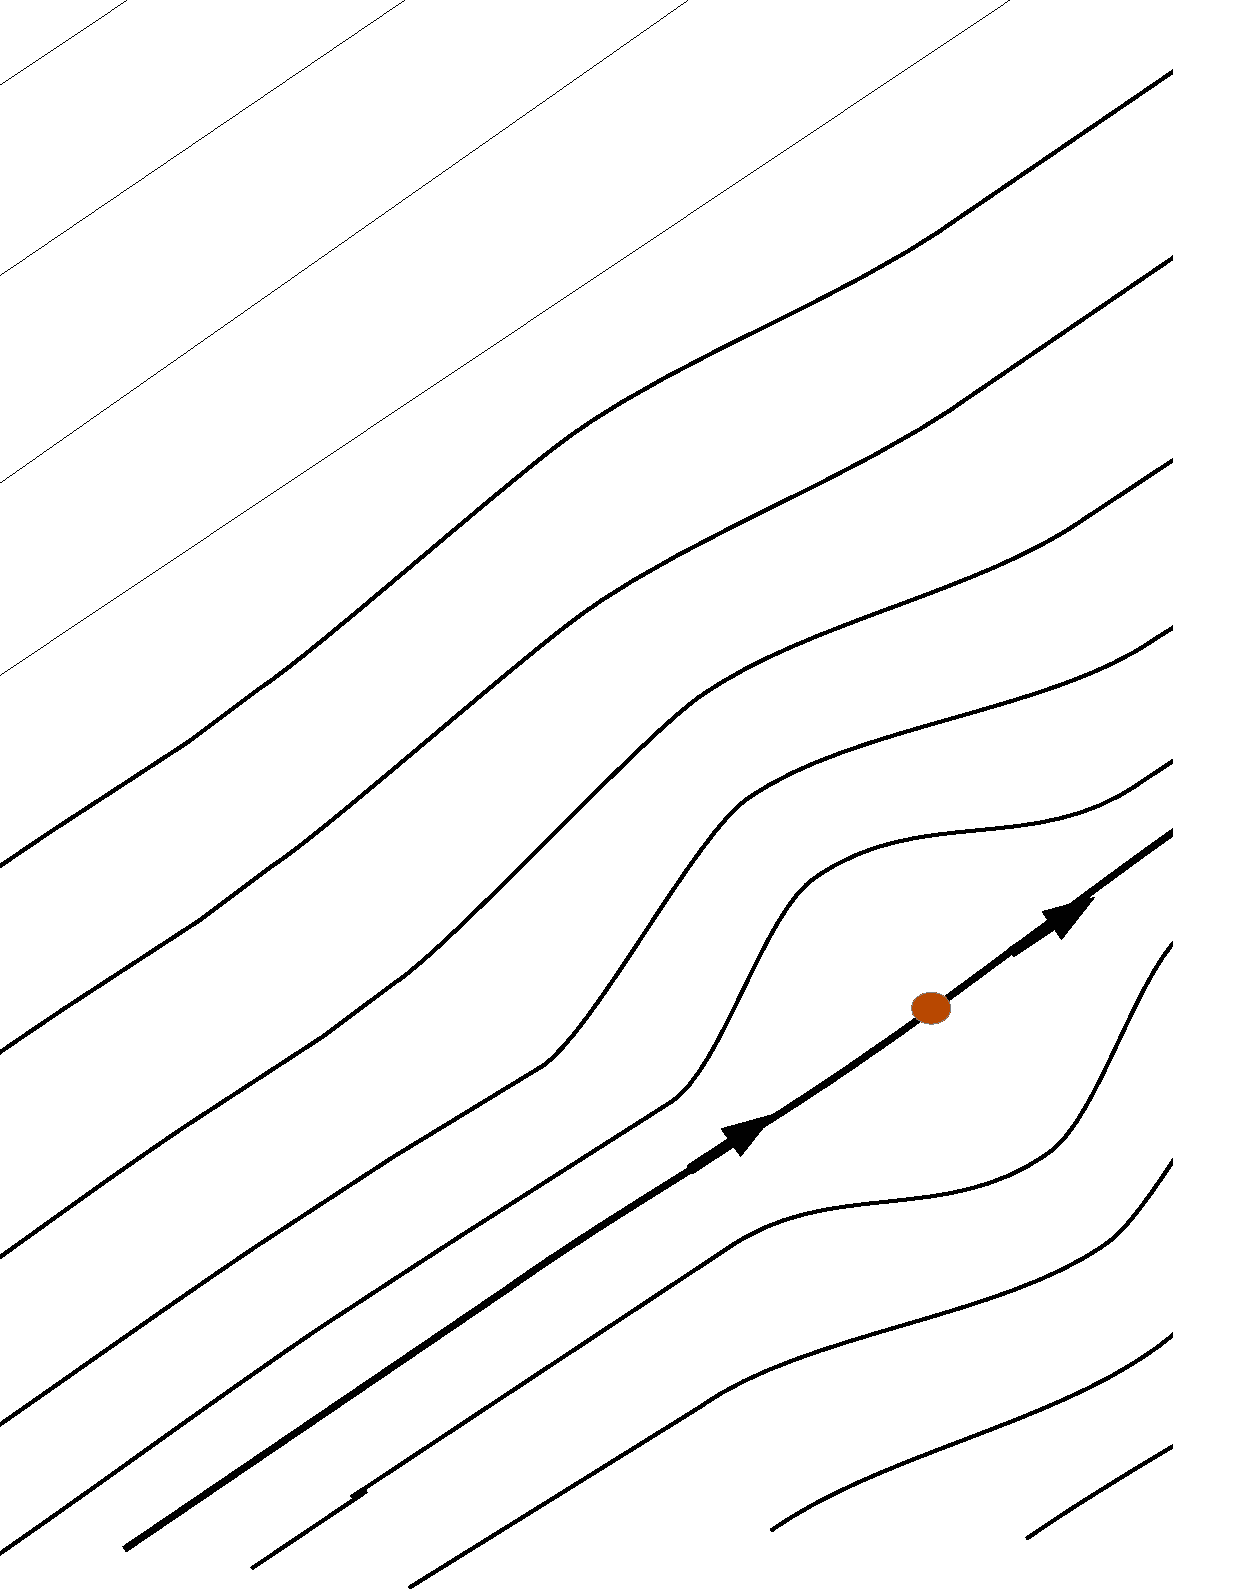
\includegraphics[scale= .15,angle=1]{kochergin4.pdf}
\caption{Torus flow with one degenerate saddle acting as a stopping point.}
\label{fig.kochergin}
\end{figure}

The Kochergin flows that we will consider have ceiling functions with power singularities of exponent $\gamma\in (0,1/2)$, and have a rotation number on the base that satisfies a full measure Diophantine type condition.

For the fiber dynamics, following \cite{DDKN}, we only need the property of exponential mixing of all orders.
A classical example of an analytic $\R^d$ action which is exponentially mixing of all orders is the \emph{Weyl chamber flow}: Let $d\geq 1$ and let $\Gamma$ be a co-compact lattice in $\SL(d+1,\R)$. Let $D_+$ be the group of diagonal matrices in $\SL(d+1,\R)$ with positive elements on the diagonal acting on $\SL(d+1,\R)/\Gamma$ by left translation. Then~$D_+$ is an $\R^d$ action that preserves the Haar measure $\nu$ on $\SL(d+1,\R)/\Gamma$ and that is exponentially mixing of all orders see \eg \cite{BEG}. Hence, we can take $G_t$ to be $D_+$.

We are ready now to give a more explicit statement of Theorem \ref{thm:main2} that will be made more precise in Section \ref{sec.koc} after Kochergin flows are precisely defined. We denote~$\mu$ the Lebesgue measure on $\T^2$ and by $\lambda$ the Lebesgue measure on $\T$.

\begin{Main} \label{thm:main22} There exists $N\in \N$ and a Kochergin flow $(K_T,\T^2,\mu)$,
with $N$ singularities and a function $\tau=(\tau_1,\ldots,\tau_{N}) \in C^\omega(\T^2,\R^{N})$ such that $\mu(\tau_i)=0$, for every $i\in [1,N]$, and such that the flow
$(F_T)\in C^\omega(\T^2\times (\SL(N+1,\R)/\Gamma),\mu\times \nu)$
defined by $F_T(x,y)=(K_T(x),G_{\tau_T(x)}y)$
satisfies the classical CLT.
\end{Main}

The dimension of the manifold on which our examples are constructed depends thus on the number of singularities $N$ that we require for the Kochergin flow. We did not try to optimize this number, but the one we currently have is of order 100.

In the next section we will define the class of {\it parabolic systems with small deviations} and recall the criterion given in \cite{DDKN} that establishes the classical CLT for skew products above a parabolic system with small deviations, provided the fiber dynamics are exponentially mixing of all orders. This part is essentially the same as in \cite{DDKN}. In a nutshell, {\it parabolic flows with small deviations} are conservative flows for which the deviations of Birkhoff averages are $o(\sqrt{T})$, but for which there exists $d \in \N^*$, and $d$-dimensional observables whose Birkhoff averages deviate, for every $T$, by more than $(\ln T)^2$ outside exceptional sets of measure less $o(T^{-5})$.

We will show that Kochergin flows on the two-torus, with exponent $\gamma\in (0,1/2)$ for the singularities of their ceiling function, and with $N(\gamma)$ singularities, are parabolic with small deviations for typical positions of the singularities and the slope of the flow.

The exponent of a singularity of the ceiling function is related to the order of degeneracy of the corresponding saddle point on $\T^2$. Limiting the order of degeneracy of the saddles thus limits the exponents to be strictly less than $1/2$. This is important to guarantee that the deviations of the Birkhoff averages above the Kochergin flow to be $o(\sqrt{T})$.

The trickiest part of the construction will be to show that if the number of saddles is sufficiently large then we can construct a smooth observable $\tau\in C^\omega(\T^2,\R^{N})$ whose Birkhoff averages above the Kochergin flow deviate by more than $(\ln T)^2$ outside exceptional sets of measure less $o(T^{-5})$.

The Diophantine property imposed on rotation angle
$\ba$ plays a crucial role in insuring refined estimates on Birkhoff sums of functions with singularities above the circular rotation of angle $\ba$, which in turn can be used to control the Birkhoff sums of observables above the Kochergin flow. Here again, we did not seek to optimize the Diophantine condition but just made sure it is of full measure.

It turns out that in finite smoothness $C^r$, certain ergodic rotations on high dimensional tori (the dimension of the torus goes to $\infty$ with $r$) are examples of diffeomorphisms that satisfy the two conditions on the deviations of the Birkhoff averages, in~fact they are \emph{parabolic with small deviations}. For this reason, they could be used in~\cite{DDKN} to construct examples of CLT diffeomorphisms with zero entropy in finite smoothness.

\subsubsection*{Acknowledgements}
The authors would like to thank to anonymous referees for comments regarding the paper.

\section{CLT for skew-products above parabolic systems with small deviations}
\label{ScCLT-Par}

In this section, we describe general conditions on the flow $(K_T,X,\mu)$ which will allow us to construct a generalized $(T,T^{-1})$ flow $(F_T)$ as in Definition \ref{def:TTinv} that satisfies the assumptions of Theorem \ref{thm:main2}.

\begin{definition}\label{def:parflow} Let $(K_T)_{T\in \R}$ be a $C^r$-flow on a manifold $X$ preserving a smooth measure $\mu$. We say that $(K_T)$ is \emph{$C^r$-parabolic with small deviations}
if the following conditions are satisfied:
\begin{enumerate}\renewcommand{\theenumi}{\textup{S}\arabic{enumi}}
\item\label{S1}
for every $H\in C^r(X)$ with $\mu(H)=0$$,
\frac{1}{\sqrt{T}}\int_0^T H(K_t\cdot )dt \Rightarrow 0$,
in distribution as $T\to\infty$.
\item\label{S2}
there exist $C,d\in \N$ and a $C^r$ function ${\btau}=(\tau_1,\ldots,\tau_d):X\to \R^d$, $\mu(\btau)=0$ such that
\[
\mu\Big(\{x\in X\;:\; \Big|\int_0^T\btau(K_tx)dt\Big|<C\ln^2 T \}\Big)=o(T^{-5}).
\]
\item\label{S3}
there exist $C>0, m <1.1$ and $x_0\in X$ such that for every $\delta>0$ sufficiently small, we have
$\DS
K_tB(x_0,\delta)\cap B(x_0,\delta)=\emptyset
$
for every $|t|\in (C\delta, (C\delta)^{-1/m})$.
\end{enumerate}
\end{definition}

Conditions \eqref{S1} and \eqref{S2} are used to show that the associated $(T,T^{-1})$-flow satisfies the classical CLT (with the possibility that the variance is identically zero). Condition~\eqref{S3}
insures that there exists a function with non-zero variance.

The following result based on \cite[Th.\,3.2]{DDKN} reduces the proof of
Theorems \ref{thm:main2} and \ref{thm:main22} to that of finding smooth parabolic flows with small deviations.

\begin{proposition}\label{prop:1} Assume that $(K_T,X,\zeta)$ is a $C^\infty$- parabolic flow with small deviations and of zero metric entropy. Let $(G_t,Y,\nu)$ be a smooth $\R^d$ action which is exponentially mixing of all orders. Let
\[
F_T(x,y)=(K_Tx, G_{\btau_T(x)}(y)),
\] where $\btau$ is as in \eqref{S2}. Then $(F_T,X\times Y,\mu \times \nu)$ has zero metric entropy and satisfies the classical CLT. Moreover, there exists $H\in C^\infty(X\times Y)$ with $\sigma^2(H)\neq 0$.
\end{proposition}
\begin{proof}
$F_T$ has zero entropy due to \cite[Lem.\,2.1]{DDKN}.
\eqref{S1} and \eqref{S2} imply that $F_T$ satisfies the classical CLT due to
\cite[Th.\,3.2]{DDKN}.
The fact that the variance is not identically zero follows from \eqref{S3} similarly
to the proof of \cite[Lem.\,8.2]{DDKN}.
\end{proof}

Let us comment on how conditions \eqref{S1} and \eqref{S2} are used in the proof of \cite[Th.\,3.2]{DDKN}. We split an arbitrary
$H\in C^r(X\times Y)$ as $H(x,y)=\bar{H}(x)+\tilde{H}(x,y)$,
where $\int H(x,y) d\nu(y)=0$ for each $x\in X$.
The ergodic integrals of $\bar{H}$ are negligible due to assumption \eqref{S1}.
To handle the integrals of $\tilde{H}$ we apply the Central Limit Theorem
for arrays over exponentially mixing actions proved in \cite{BG}.
This theorem establishes asymptotic normality of
$\cS_T(y):=\int_{\reals^d} \bA_t(G_t y) d\fm_T(t)$,
where the norms of $\bA_t$ are uniformly bounded and the measures
$\fm_L$ satisfy the following free conditions:

\begin{enumeratea}
\item\label{enum:a}
$\lim_{T\to\infty}
\fm_T(\R^d)=\infty$.

\item\label{enum:b}
For each $r\in \naturals$, $r\geq 3$, and each $K>0$,\vspace*{-3pt}
\[
\lim_{T\to \infty} \int \fm_T^{r-1}\Big(B(t,K\ln \fm_T(\reals^d))\Big) d\fm_T(t)=0,
\]
where $B(t,v)$ denotes a ball in $\R^d$ of radius $v>0$ centered at $t$.

\item\label{enum:c}
There exists $\sigma^2=\sigma^2(\bA_t)\geq 0 $ so that $\DS \lim_{T\to \infty} V_T=\sigma^2$, where\vspace*{-3pt}\enlargethispage{.5\baselineskip}
\[
V_T:=\int\cS_T^2(y)d\nu(y)= \iiint \bA_{t_1} (G_{t_1} y) \bA_{t_2} (G_{t_2} y) d\fm_T (t_1)
d\fm_T(t_2) d\nu(y).
\]
\end{enumeratea}

To prove \cite[Th.\,3.2]{DDKN}, we apply this result with $\fm_T$ being the normalized occupation measure $\fm_T(\Omega)=\mes(t\leq T: \tau_t(x)\in \Omega)/\sqrt{T}$.
Then \eqref{enum:a} holds since $\fm_T(\reals^d)=\sqrt{T}$, \eqref{enum:c} holds due to the ergodic theorem
(see \cite[\S 5.1.2]{DDKN} for details),
and
\eqref{S2} is used to verify \eqref{enum:b} since it implies that $\tau_{t_1}(x)$ and $\tau_{t_2}(x)$ are
unlikely to be close unless~$t_1$ and~$t_2$ are close (see \cite[\S 5.1.2]{DDKN} for details).

As explained in the introduction a classical example of an analytic $\R^d$ action which is exponentially mixing of all orders is the \emph{Weyl chamber flow}. It remains to find examples of smooth flows with small deviations.
In light of Proposition \ref{prop:1}, Theorem~\ref{thm:main2} becomes an immediate consequence of the following result:

\begin{Main}\label{thm:SP} There exists a smooth conservative flow $(K_T,X,\mu)$ with zero metric entropy that is a parabolic flow with small deviations.
\end{Main}

Theorem \ref{thm:SP} is the main novelty of this work. Existence of $C^\infty$ parabolic diffeomorphisms with small deviations is an open question. In fact, to the best of our knowledge, the following easier problem is open:
\begin{problem} Construct a $C^\infty$ diffeomorphism $f$ on a smooth compact manifold $X$ preserving a smooth measure $\mu$ such that:
\begin{enumerate}\renewcommand{\theenumi}{\textup{T}\arabic{enumi}}
\item\label{T1}
for every $H\in C^\infty (X)$ with $\mu(H)=0$ we have\vspace*{-3pt}
\[
\frac{1}{\sqrt{N}}\sum_{n\leq N} H(f^n \cdot )dt\implies 0,
\]
in distribution as $T\to\infty$;
\item\label{T2}
there exists $x\in X$ and $\phi\in C^\infty(X)$ such that
$\DS
\{\phi_n(x)\}:=\big\{\sum_{n\leq N} \phi(f^nx)\big\} $
is unbounded.
\end{enumerate}
\end{problem}

In other words, in all the known smooth examples, whenever there exists a zero average function which is not a coboundary (equivalently \eqref{T2} holds) then there is a rapid jump in asymptotics of ergodic averages, \ie they become of order $\sqrt{N}$ or larger. Hence, in light of Katok's conjecture on cohomologically rigid diffeomorphisms, one can ask the following:

\emph{Does there exist a $C^\infty$ diffeomorphism $f$ on a smooth compact manifold $X$ preserving a smooth measure $\mu$, not conjugated to a Diophantine torus translation},
so that \eqref{T1} holds?

It is interesting to point out that the classical parabolic flows,including horocycle flows and their reparametrizations, nilflows and their reparametrizations, \emph{are not} parabolic with small deviations. Indeed, it follows from the work of Flaminio-Forni, \cite{Fla-Fo} and \cite{Fla-Fo2}, that the deviations of ergodic averages in these examples are, for observables that are not coboundaries, of order at least $\sqrt{T}$ for a positive measure set of points.
Thus property \eqref{T1} does not hold for those flows.
Moreover, these flows are known not to have a CLT and it is therefore not possible to use them to construct skew products above them that satisfy the classical CLT.

{Finally, let us mention that another way for constructing smooth conservative flows or diffeomorphisms with zero entropy and a classical CLT would be to look for zero entropy systems having a polynomial speed of mixing faster than $T^{-a}, a>1$. To the best of our knowledge, such systems are not yet proved to exist.}

The rest of the paper is devoted to the proof of Theorem \ref{thm:SP}. Our examples
belong to the class of smooth flows on surfaces with degenerate saddles (so called \emph{Kochergin flows}).

For the class of Kochergin flows that we consider all the singularities will be ``weakly'' degenerate, \ie the strength of the singularity will be $o(x^{-1/2})$. This assumption will relatively easily give us the condition \eqref{S1} for any number of singularities. Condition \eqref{S3} will also be easy to achieve by assuming that the base rotation (the first return map) is Diophantine. The most interesting and also most difficult part is to show existence of $\btau$ satisfying the assumptions of \eqref{S2}.

\section{Construction of parabolic Kochergin flows in the smooth case} \label{sec.koc}

\subsection{Overview of the construction}
\label{SSOverview}

We start by defining $C^\infty$ Kochergin flows on~$\T^2$. They were introduced by Kochergin in \cite{Koch}.
{ Namely,}
\cite{Koch} takes a linear flow on~$\T^2$ in direction $(\alpha,1)$ and cuts out finitely many disjoint disc from the phase space. Inside each such disc one then glues in a \emph{Hamiltonian flow} on $\R^2$ with a degenerated singularity at $\bar{c}\in \T^2$ (corresponding to $(0,0)\in \R^2$). Finally one smoothly glues the trajectories of the linear flow with the trajectories of the Hamiltonian flow. It follows that each such flow preserves a smooth area measure on $\T^2$. Moreover, as shown by Kochergin, such flows are mixing for all irrational $\alpha\in \T$. For more details on the construction we refer the reader to \cite{Koch}. In our case we will cut out finitely many discs centered at
$\{\bar{c}_i\}_{i=1}^N$ and glue a Hamiltonian flow with a degenerated singularity at $0$ in the discs centered at points $\{\bar{c}_i\}_{i=1}^N$. From the construction it follows that the set $\cT=\T\times\{0\}$ is a global transversal for the flow (we can WLOG assume that no discs intersects $\cT$) and moreover the first return map is the rotation by $\alpha\in \T$. The roof function $f:\T\to \R_+$ (first return time) is smooth except at { the points $\{c_i\}_{i=1}^N$ which are the projections (to $\cT$) along the flow lines of the points $\{\bar{c}_i\}_{i=1}^N$}and at which the roof function has a power-like singularity with exponent $\gamma \in (0,1)$.

In what follows, when we write $\{c_i\}_{i=1}^N\subset \cT$, we allow singularities of the smooth flow $(K_t)$ to be anywhere on the unit flow lines of the linear flow in direction $\alpha$, \ie $\bar{c_i}=L^{\alpha}_{t_i}(c_i,0)$ with $0<t_i<1$ and where $(L^\alpha_t)$ denotes the linear flow on $\T^2$ in direction $(\alpha,1)$.
In fact we will construct \emph{good} tuples of points $(c_1,\ldots, c_N)$ and then we lift them along the flow as described above.

In particular, every point in $x\in M$ which is not a fixed point can be written as $x=K_w \theta$, where $\theta\in \cT$ and $0\leq w<f(\theta)$. By the construction it follows that
\begin{equation}\label{fsum}
f(\cdot)=\sum_{i=1}^N\, \bar{f}(\cdot-c_i),
\end{equation}
where $c_i\in \cT$ denote the projections of $\bar{c}_i\in \T^2$ along the flow lines, where, as shown in \cite{Koch}, $\bar{f}:\T\to \R_+$ is $C^3$ on $\Tor\setminus\{0\}$, satisfies
$\int \bar f d \lambda = 1$ and
\begin{equation}\label{eq:asy2}
\lim_{\theta\to 0^+}\frac{\bar{f}{}''(\theta)}{\theta^{-2-\gamma}}=A=
\lim_{\theta\to 1^-}\frac{\bar{f}{}''(\theta)}{(1-\theta)^{-2-\gamma}},
\end{equation}
where $A>0$ and $\gamma\in (0,1)$. In this context Kochergin showed that $\gamma=1/3$ is a possible exponent. For simplicity we will always assume that \eqref{eq:asy2} holds with
$A=1$. Let us denote $\mathcal{K}(\alpha,\gamma, \{c_i\})$ the set of smooth area preserving flows $(K_t)$ on $\T^2$ for which~$R_\alpha$ is the first return map and the corresponding first return time $f$ satisfies~\eqref{fsum} where~$\bar{f}$ satisfies \eqref{eq:asy2}. In what follows we will always assume that $\gamma<1/2$.

Thus Kochergin flows are isomorphic to special flows defined as follows.
The orbit of a point $(\theta,u)$, $\theta \in \T$, $u\in [0,f(\theta))$ under the flow $(K_T)$ for positive time $t$ is given~by
\begin{equation}\label{eq.special}
K_t(\theta, u)=(\theta+n\alpha, u+t-S_n(f)(\theta)),
\end{equation}
where $S_n(f)$ is the ergodic sum of $f$ and $n((\theta,u),t)$ is the unique integer such that $0\leq u+t-S_n(f)(\theta)<f(\theta+n\alpha)$. The orbits for negative times are defined similarly. Let $C=(\inf_\T f)^{-1}$. Notice that $n((\theta,u),t)\leq C|t|$.

\begin{figure}[htb]
\centering
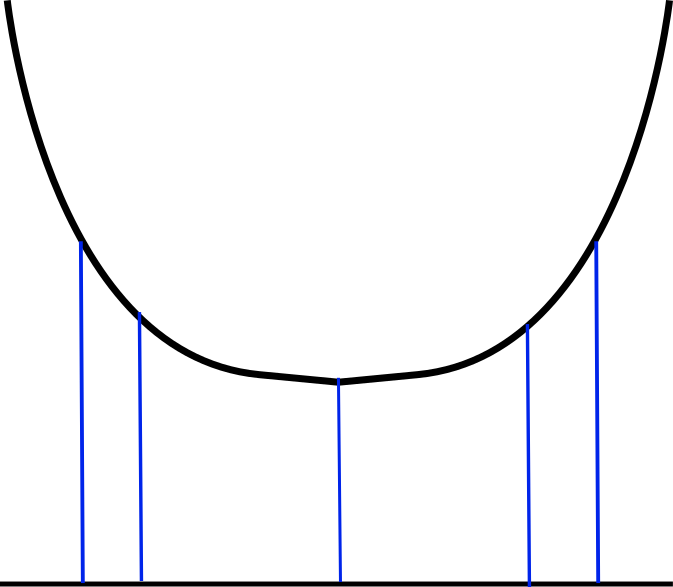
\includegraphics[scale=.2,angle=0]{symetric.png}
\caption{Representation of a $2$-torus flow with one degenerate saddle as a special flow under a ceiling function with a power-like singularity.}
\label{sym}
\end{figure}

Let $(a_n)$ denote the continued fraction expansion of $\alpha$ and $(q_n)$ denote the sequence of its denominators, \ie $q_0=q_1=1$ and
\begin{equation*}%\label{eq:qi}
q_{n+1}=a_{n+1}q_n+q_{n-1}.
\end{equation*}
Let
\begin{equation}\label{eq:cp}
\cD:=\{\alpha\in \T\;:\;\exists C>0 \; \text{ such that }q_{n+1}<Cq_n \ln^2 q_n \text{ for every }n\in \N\}.
\end{equation}
The set $\cD$ has full measure by Khintchine's theorem, \cite[\S 13]{Khi}. The following statement
gives explicit examples of flows that satisfy Theorem \ref{thm:SP}.
\begin{Main}\label{prop:sch} For every $\alpha\in \cD$ and every $\gamma<1/2$, there exists $s\in \N$ and a full measure set $\cC\subset [0,1]^s$ such that for every $(c_1,\ldots, c_s)\in \cC$, every $C^r$ flow in $\mathcal{K}(\alpha,\gamma, \{c_i\})$
with $r\geq 3$ is $C^r$- parabolic with small deviations.
\end{Main}
In the above theorem $r$ may be equal to $\infty$ or $\omega$. We also point out that the following stronger result holds: when $r=\omega$, condition \eqref{S1} will still be satisfied for all $C^3$ functions.
Theorem \ref{prop:sch} is a direct consequence of the following two results.

\begin{proposition}\label{lem:sch2} For every $s\in \N$, every $(c_1,\ldots, c_s)\in [0,1]^s$, every $\alpha\in \cD$ and every $\gamma<1/2$ every smooth flow in $\mathcal{K}(\alpha,\gamma, \{c_i\})$ satisfies properties \eqref{S1} and \eqref{S3}.
\end{proposition}

\begin{proposition}\label{prop:sch2}
For every $\alpha\in \cD$ and every $\gamma<1/2$ there exists $s\in \N$ and a full measure set $\cC\subset [0,1]^s$ such that for every $(c_1,\ldots, c_s)\in \cC$, every smooth flow in $\mathcal{K}(\alpha,\gamma, \{c_i\})$ satisfies \eqref{S2}.
\end{proposition}

We will now prove Proposition \ref{lem:sch2}.
\begin{proof}[Proof of Proposition \ref{lem:sch2}] We first show \eqref{S3}. we consider the representation of $K_t$ as a special flow over a rotation as in \eqref{eq.special}.
We have
\[
K_t(\theta, u)=(\theta+n\alpha, u+t-S_n(f)(\theta))
\]
for some $|n|\leq C |t|$ where $S_n(f)$ is the ergodic sum of $f$. Let $x_0=(\theta,u)$ be any point which is not a fixed point of the flow.
If $n=0$, then \eqref{S3} holds since the second coordinates differ by at least $C\delta$, (as the vector field is positive since $x_0$ is not a fixed point).
{ If $n\neq 0$ then the first coordinates differ by at least $\|n\alpha\|$. Since $\alpha\in \cD$ it follows that there is a constant $C_\alpha>0$ such that $\|n\alpha\|\geq \sfrac{C_\alpha}{n \log^4 n}$. In particular, the first coordinates of $K_t(\theta,u)$ and $(\theta,u)$ differ by at least $\sfrac{C'}{t \log^4 t}$ (as $|n|\leq C|t|$). It is enough to take $m=1/2$ (or in fact any fixed $m<1$) to get \eqref{S3}.}

Property \eqref{S1} was proved in \cite{DDKN} in case there is just one singularity (\ie $N=1$). However the proof works with minor changes for multiple singularities. Alternatively, one can also use \cite[Th.\,1.1]{FM} in the context of surfaces of genus $1$. In this case the asymptotic growth in $L^1$ is given in \cite[Eq.\,(1.5)]{FM} ({Note that $b(\sigma,|\alpha|)$ appearing in right-hand side of that formula
equals to $\gamma<\sfrac{1}{2}$ for the case considered in our paper}).
\end{proof}

The proof of Proposition \ref{prop:sch2} is the most important part of the paper. The rest of Section \ref{sec.koc} as well as Section \ref{ScTechnical} is devoted to its proof.

\begin{itemize}
\item
In Section \ref{sec.preliminaries}, we give useful estimates on ergodic sums of functions with singularities above circular rotations of frequency $\alpha \in \cD$.

\item
In Section \ref{sec.singularities}, we give the criteria along which the singularities should be selected. We state Proposition \ref{prop.choice.c} that says that, under the condition $\alpha \in \cD$, the typical choice of the singularities satisfies the criteria.

\item
In Section \ref{sec.tau.choice}, we explain how the cocycle $\tau$ must be chosen. We state the main part of the proof, Proposition \ref{prop.choice.tau} that says that the chosen cocycle satisfies \eqref{S2}.

\item
In Section \ref{sec.c.choice}, we prove Proposition \ref{prop.choice.c} and in Section \ref{SSprop.choice.tau} we prove Proposition~\ref{prop.choice.tau}.
\end{itemize}

\Subsection{Preliminary estimates on ergodic sums of functions with singularities} \label{sec.preliminaries}

\begin{lemma}\label{lem:DK0}Let $\bar{f}$ be as in \eqref{eq:asy2}. Then for every $N\in \N$ and every $x\in \T$
\[
\biggl|S_N(\bar{f})(x)- N\int_\T \bar{f}d \lambda-\bar{f}(x_{\min,N})\biggr|={\rm O}(N^\gamma\ln^{5} N),
\]
where $x_{\min,N}=\DS \min_{0\leq j<N} \|x+j\alpha\|$.
\end{lemma}

\begin{proof}
This follows from the assumptions on $\alpha$ and from \cite[Prop.\,5.2]{CW}.
In~fact, \cite[Prop.\,5.2]{CW} is proved for monotone observables,
but by our assumptions \eqref{eq:asy2} we can write $\bar{f}=g+h$ where $g$ is monotone and satisfies \eqref{eq:asy2} and $h$ is of bounded variation.
The ergodic sums of $g$ are ${\rm O}(N^\gamma\ln^{5} N)$ by \cite{CW}
while the ergodic sums of $h$ are $O(\ln^4 N)$ by Lemma \ref{LmSumBV}
{from the appendix}.
\end{proof}

We want to describe the set where ergodic sums of the function $\bar{f}$ satisfying \eqref{eq:asy2} are small. For small enough $\eps>0$ let
\begin{equation}\label{eq:an0}
A_N:=\{x\in \T\;:\; |S_N(\bar{f}_0)(x)|\leq N^{\gamma^2+\eps}\},
\end{equation}
where $\bar{f}_0=\bar{f}-\int_\T \bar{f} d \lambda$.

The rest of this section is devoted to the proof of the following:

\begin{proposition} \label{lemma.delta}
Let $\delta_N=\sfrac{1}{N^{1+\gamma/5}}$. There are $a_1,\ldots a_{3N}\in \T$ such that
\begin{equation}\label{eq:an}
A_N\subset \bigcup_{i=1}^{3N}(-\delta_N+a_i,a_i+\delta_N)
\end{equation}
holds for every sufficiently large $N\in \N$.
\end{proposition}
\begin{proof}
Let $\bar{f}$ be as in \eqref{eq:asy2}. First we state the following lemma giving lower bounds on the size of $\bar{f}{}''$:
\begin{lemma}\label{lem:DK} For sufficiently large $N\in \N$ and for every $x\in \T\setminus\{-i\alpha\}_{i=0}^{N-1}$ we have
\[
S_N(\bar{f}{}'')(x)\geq N^{2+\gamma}\ln^{-10}N.
\]
\end{lemma}
\begin{proof} { Notice that by the fact that $A>0$ in \eqref{eq:asy2} it follows that there is a $\kappa_0>0$ such that $\bar{f}{}''$ is positive on $[0,\kappa_0)\cup (1-\kappa_0,1)$. In particular there exists $C>0$ such that for any $0\leq j<N$ and any $x\in \T$, $S_N(\bar{f}{}'')(x)\geq \bar{f}{}''(x+j\alpha)- C N$. We use it for~$j$ which minimizes the $\|x+s\alpha\|$ over $0\leq s<N$, \ie $x+j\alpha=x^N_{\min}$}. It follows that if $n$ is such that $N\in [q_n,q_{n+1})$, then $0<x^N_{\min}<\sfrac{1}{q_n}$. Then the statement follows from \eqref{eq:asy2} and the Diophantine assumption on $\alpha$ as
\[
q_n^{2+\gamma}\geq q_{n+1}^{2+\gamma}\ln^{-8}(q_{n+1})\geq N^{2+\gamma}\ln^{-8}N.\qedhere
\]
\end{proof}

Consider the interval partition $\cP_N$ of $\T$ by points $\{-i\alpha\}_{i=0}^{N-1}$. Then by \eqref{eq:asy2} it follows that $S_N(\bar{f}_0)(\cdot)$ is a $C^3$ function on Int$(I_j)$ for every interval $I_j\in \cP_N$. Let $I_j=[a_j,b_j)$. By Lemma \ref{lem:DK} it follows that $S_N(\bar{f}{}')(\cdot)$ is monotone on $I_j$. By de~l'Hôpital's rule
$S_N(\bar{f}{}'_0)(\cdot)$ satisfies $\DS \lim_{x\to a_j^+}S_N(\bar{f}{}'_0)(x)=-\infty$ and
$\DS \lim_{x\to b_j^-}S_N(\bar{f}{}'_0)(x)=\infty$. So~let $a_{j,1}=y_j\in I_j$ be the unique
point such that $S_N(\bar{f}{}'_0)(a_{j,1})=0$. Note that
\[
S_N(\bar{f}{}'_0)(x)-S_N(\bar{f}{}'_0)(a_{j,1})=S_N(\bar{f}{}''_0)(\theta_x)(x-a_{j,1}).
\]
In particular, if $J_{j,0}$ is an interval of size $\sfrac{2}{N^{1+\gamma/5}}$ centered at $a_{j,1}$, by Lemma \ref{lem:DK} it follows that for $x\in I_j\setminus J_{j,0}$
\begin{equation}\label{eq:sm1}
|S_N(\bar{f}{}'_0)(x)|\geq N^{2+\gamma}\ln^{-10}N \cdot \frac{1}{N^{1+\gamma/5}}= N^{1+4\gamma/5}\ln^{-10}N.
\end{equation}
Consider the two disjoint intervals $K_{j,1}$ and $K_{j,2}$ in $I_j$ so that $K_{j,1}\cup K_{j,2}=I_j\setminus J_{j,0}$. Then for $w=1,2$, let $x_{j,w}\in K_{j,w}$ be the point minimizing $S_N(\bar{f}_0)(\cdot)$ on $K_{j,w}$. If~$S_N(\bar{f}_0)(x_{j,w})\geq N^{\gamma^2+\eps}$, then $A_N\cap I_j\subset J_{i,0}$. If not, let $J_{j,w}$ be an interval of size $\sfrac{2}{N^{1+\gamma/5}}$ centered at $x_{j,w}$. Then for every $x\in K_{j,w}$, we get
\[
|S_N(\bar{f}_0)(x)-S_N(\bar{f}_0)(x_{j,w})|=|S_N(\bar{f}{}'_0)(\theta_x||x-x_{j,w}|
\]
for some $\theta_x\in K_{j,w}$. So if $x\in K_{j,w}\setminus J_{j,w}$, then by \eqref{eq:sm1} we get
\begin{align*}
|S_N(\bar{f}_0)(x)|&\geq N^{1+4\gamma/5}\ln^{-10}N\cdot \frac{1}{N^{1+\gamma/5}}- S_N(\bar{f}_0)(x_{j,w})\\
&\geq N^{3\gamma/5}\ln^{-10}N -N^{\gamma^2+\eps}>N^{\gamma^2+\eps},
\end{align*}
if $\eps>0$ is small enough (remember that $\gamma<1/2$). It then follows that
\[
A_N\cap I_j\subset J_{j,1}\cup J_{j,2}\cup J_{j,0}.
\]
and the $J_{j,w}$ are intervals of size $\sfrac{2}{N^{1+\gamma/5}}$ centered at $a_{j,w}$. Then
\[
A_N\subset \bigcup_{j=1}^N[J_{j,1}\cup J_{j,2}\cup J_{j,0}].
\]
This gives \eqref{eq:an} and finishes the proof.
\end{proof}

\subsection{Choosing the singularities} \label{sec.singularities}
We will consider a Kochergin flow $(K_t)$ with $\gamma<1/2$, $\alpha\in \cD$, and a roof function $f$ given by
\begin{equation*}%\label{fsum'}
f(\cdot)=\sum_{i=1}^{s+3} \bar{f}(\cdot-c_i),
\end{equation*}
where $s:=\lfloor \sfrac{50}{\gamma} \rfloor$. In this subsection we describe the choice of the $c_i\in \cT$.
In the process, we will explain why it is preferable for the presentation to index the singularities from $1$ to $s+3$ instead of from $1$ to $s$ with a larger $s$.

For $\bar{c}\in \T^2$ let $V_\kappa (\bar{c})$ be the ball of radius $\kappa>0$ centered at $\bar{c}$.
Recall that $A_N$ is defined in \eqref{eq:an0} as
$
\DS A_N:=\{x\in \T\;:\; |S_N(\bar{f}_0)(x)|\leq N^{\gamma^2+\eps}\}$.

For $n\in \N$ and $c\in \T$ let
\begin{equation}\label{eq:gcn}
G(c,n)= \bigcup_{\Z\ni k=-2q_{n+1}}^{2q_{n+1}}
R^k_\alpha\Bigl[c-\frac{1}{q_n\ln^{5}q_n}, c+\frac{1}{q_n\ln^{5}q_n}\Bigr].
\end{equation}

Let $S(T,(i_v)_{v=1}^s)$ be the set of points $\bx=(x, w)$ such that
\begin{equation}\label{eq:awaysing}
\{\bx, K_T(\bx)\}\cap \bigcup_{j\in \{i_1,\ldots,{i_s}\} }V_\kappa(\bar{c}_j)
{=\emptyset}
\end{equation}
and
\begin{multline}\label{eq:awaysing2}
\{x+N(x,w,T)\alpha+u\alpha\}_{|u|\leq 2T^\gamma, u\in \Z} \\
\cap
\bigcup_{j\in \{i_1,\ldots,{ i_s}\}} \Big[-\frac{1}{2T^\gamma\ln^{7}T}+ c_j, c_j+\frac{1}{2T^\gamma\ln^{7}T}\Big]
=\emptyset.
\end{multline}

\begin{definition} \label{def.good}
We say that the set of singularities $\{c_1,\ldots,c_{s+3}\}$ is {\it good} if
\begin{enumerate}\renewcommand{\theenumi}{$\cG$\arabic{enumi}}
\item\label{cG1}
for every $i,j \in \{1,\ldots, s+3\}$, for any $n$ sufficiently large
\[
G(c_i,n)\cap G(c_j,n)=\emptyset,
\]

\item\label{cG2}
for any choice of pairwise different elements $i_1,\ldots,i_s$ from $\{1,\ldots,s+3\}$ and for $N$ sufficiently large
\[
\lambda\Big(\bigcap_{w=1}^sA_N+c_{i_w}\Big)\leq N^{-6},
\]

\item\label{cG3}
for sufficiently large $T\!>\!0$, for every $\bx\!\in\! \T^2$ there is \hbox{$(i_1,\ldots,i_s)\!\subset\! \{1,\ldots,s+3\}$} such that $ \bx\in S(T,(i_v)_{v=1}^s)$.
\end{enumerate}
The set of good tuples will be denoted by $\cC$.
\end{definition}

{ Let us shortly explain how the above properties are used. Property \eqref{cG1} implies that the orbit of any point $\bx$ and any time $T$ can visit at most one of the neighborhoods of the $\{c_j\}$, \ie if the orbit goes very close to $c_i$ then it stays at a controlled distance away from all the other $c_j$ with $j\neq i$. Property \eqref{cG2} implies that if we define the roof function $f$ to have singularities at the $\{c_j\}$, then for most points (except a set of measure $N^{-6}$) the ergodic sums up to time $N$ of $f$ will be polynomially large. Here is where we use that we have more singularities -- each of them produces a bad set of measure $\leq N^{-\delta_0}$ and we roughly show that the bad sets are independent for our choice of singularities. Property \eqref{cG3} implies that for a short orbit (of size $T^\gamma$) of every point $\bx$ does not enter the ball of radius $T^{-\gamma}\ln^{-7}T$ centered at $c_i$ for at least~$s$ indices $i$.}

\medskip
\begin{remark}\label{rem:toadd} Notice that by property \eqref{cG1} and the Diophantine assumptions on $\alpha$ it follows that for any $i,j\in \{1,\ldots, s+3\}$, and any $0<|u|\leq M$ (with $M$ sufficiently large)
\[
\|c_i-c_j+u\alpha\|\geq \frac{1}{M\log^{20}M}.
\]
Indeed, if $n$ is the largest for which $M\leq q_{n+1}$, then by \eqref{cG1} it follows that
\[
\|c_i-c_j+u\alpha\|\geq \frac{1}{2q_n\log^5 q_n}\geq \frac{1}{M\log^{20}M},
\]
the last inequality by the Diophantine assumption on $\alpha$.
\end{remark}

The reason why we preferred to index the singularities from $1$ to $s+3$ is that we need, for each
$\bx$ and every $T$, that there exist at least $s$ singularities such that \eqref{cG3} holds. In Lemma \ref{lem:sep}, we will see why considering $s+3$ singularities instead of $s$ is sufficient for insuring \eqref{cG3}.

The choice of the singularities $c_1,\ldots,c_{s+3}$ is based on the following result that we will prove in Section \ref{sec.c.choice}.

\begin{proposition} \label{prop.choice.c} For the set $\cC$ of Definition \ref{def.good}, we have
$\Leb_{s+3}(\cC)=1$.
\end{proposition}

\subsection{Choosing the cocycle $\btau$} \label{sec.tau.choice}

Define a $C^\infty$ function
\[
\btau=(\tau_1,\ldots,\tau_{s+3}):\T^2\to \R^{s+3}
\]
as follows: For $i\in\{1,\ldots, s+3\}$ let $\tau_i:\T^2\to \R$ be a $C^\infty$ mean zero function such that $\tau_i=1$ on $V_\kappa (\bar{c}_i)$ and $\tau_i=0$ on $V_\kappa(\bar{c}_j)$ with $j\neq i$, for some small $\kappa$ such that $\DS 0<\kappa<\frac{1}{2}\min_{i\neq j}\|\bar{c}_i-\bar{c}_j\|$.

\begin{proposition} \label{prop.choice.tau} Assume $(c_1,\ldots,c_{s+3})\in [0,1]^{s+3}$ are {\it good} as in Definition \ref{def.good}. Then, the flow $(K_t)$ defined as in \eqref{fsum} satisfies \eqref{S2}. More precisely, the function $\btau$ satisfies
\[\ts
\nu\Big(\{x\in \T^2\;:\; \big\|\int_0^T\btau(K_tx)dt\big\|<C\ln^2 T \}\Big)=o(T^{-5}),
\]
where $\nu$ is the Haar measure on $\T^2$.
\end{proposition}

\section{The proofs of technical propositions.}
\label{ScTechnical}
\subsection{Proof of Proposition \ref{prop.choice.c}} \label{sec.c.choice}
We will always fix $s=\lfloor \sfrac{50}{\gamma} \rfloor$.
We start with \eqref{cG1}.
\begin{lemma} \label{lemma.G1} There is a set $\cF\in [0,1]^{s+3}$ of full Lebesgue measure such that for any $(c_1,\ldots,c_{s+3})\in \cF$, for every $i,j \in \{1,\ldots, s+3\}$, for any $n$ sufficiently large
\[
G(c_i,n)\cap G(c_j,n)=\emptyset,
\]
where the sets $G(c,n)$ are as in \eqref{eq:gcn}.
\end{lemma}

\begin{proof} Define
\begin{equation}\label{eq:fn}
F_n:=\big\{(c_1,\ldots, c_{s+3})\in [0,1]^{s+3}\;:\; G(c_i,n)\cap G(c_j,n)=\emptyset, \text{ for any } i\neq j\big\}.
\end{equation}
We have the following:

\begin{claim}
For $n$ sufficiently large, we have
\[
\Leb_{s+3}(F_n)\geq 1-\frac{1}{\ln^2q_n}.
\]
\end{claim}

\begin{proof}[Proof of the claim] We say that $d\in \T$ is $n$-far from $c\in \T$ if $G(c,n)\cap G(d,n)=\emptyset$. We have
\[
\
\lambda(\{d: d \text{ is } n \text{ far from } c\}\geq 1-\frac{8q_{n+1}}{q_n\ln^5q_n}\geq 1-\frac{8{C}}{\ln^3q_n},
\] the last inequality since $\alpha\in \cD$. Notice that $F_n$ contains vectors $(c_1,\ldots,c_{s+3})\in [0,1]^{s+3}$ such that $c_1$ is any number in $[0,1]$, $c_2$ is $n$-far from $c_1$, $c_3$ is $n$-far from $c_2$ and $n$-far from $c_1$, and so on until $c_s$ is $n$-far from $c_j$ for every $j<s$. Therefore,
\[
\Leb_{s+3}(F_n)\geq \prod_{\ell=1}^{s+3} \Bigl(1-\frac{8{C}\ell}{\ln^3q_n}\Bigr)\geq 1-\ln^{-2}q_n,
\]
if $n$ is sufficiently large.
\end{proof}
Thus the set
\begin{equation*}%\label{eq:cf}
\cF:=\bigcup_{m=1}^{+\infty} \bigcap_{n\geq m}F_n
\end{equation*}
satisfies $\Leb_{s+3}(\cF)=1$ and the condition of Lemma \ref{lemma.G1}.
\end{proof}

We proceed to \eqref{cG2}.

\begin{lemma} \label{lemma.G2}There is a set
$\mathbb{D}\in [0,1]^s$ of full Lebesgue measure such that for any $(c_1,\ldots,c_s)\in \mathbb{D}$, for $N$ sufficiently large
\[
\lambda\Big(\bigcap_{i=1}^sA_N+c_{i}\Big)\leq N^{-6},
\]
where $A_N$ is as in \eqref{eq:an0}.
\end{lemma}

\begin{proof}
We have the following, where addition is mod $1$.

\begin{claim}
Let $N\in \N$, $\delta>0$, $b_1,\ldots b_N\in \T$ and let $A\subset \T$ be such that
\[
A\subset \bigcup_{i=1}^N(-\delta+b_i,b_i+\delta).
\]
Then for any $s\in \N$
\begin{equation}
\label{FewTranslates}
\int_{[0,1]^s}\lambda\Big( \bigcap_{i=1}^s(A+t_i)\Big)dt_1\ldots dt_s{\leq} (2N\delta)^{s}.
\end{equation}
\end{claim}

\begin{proof}[Proof of the claim]
The left-hand side of \eqref{FewTranslates}
equals to
\[
\int_{\T^{s+1}} \prod_{i=1}^s \chi_{-A} (t_j-x) dt_1\dots dt_s dx=\lambda(A)^s,
\]
where the equality uses the change of variables $u_j=t_j-x$ and where $\chi_W$ denotes the characteristic function of a set $W$.
\end{proof}
We now apply the claim to the sets $A_N$ defined by \eqref{eq:an0}, $\delta_N=\sfrac{1}{N^{1+\gamma/5}}$ and $s=\lfloor \sfrac{50}{\gamma} \rfloor$. Then, using Proposition \ref{lemma.delta},
\[
\int_{[0,1]^s}\lambda\Big(\bigcap_{i=1}^s(A_N+t_i)\Big)dt_1\ldots dt_s\leq N^{-9}.
\]
So by Markov's inequality the set
\[
B_N:=\Big\{(t_1,\ldots,t_s)\in [0,1]^s\;:\; \Leb_s\Big(\ts\bigcap_{i=1}^s(A_N+t_i)\Big)\leq N^{-6}\Big\}
\]
satisfies
$\DS
\Leb_s(B_N)\geq 1-\sfrac{1}{N^2}$.
We now define the set $\mathbb{D}$ as
\[
\mathbb{D}:=\bigcup_{m=1}^{+\infty} \bigcap_{N\geq m}B_N.
\]
Then $\mathbb{D}$ is a full measure subset of $[0,1]^s$ that satisfies the condition of Lemma \ref{lemma.G2}.
\end{proof}

We finally define the set $\cC$ that satisfies the requirements of
Proposition \ref{prop.choice.c}
\begin{multline*}%\label{eq:cc}
\cC:=\Big\{(c_1,\ldots,c_{s+3})\in [0,1]^{s+3}:\\
(c_{i_1},\ldots,c_{i_s})\in \mathbb{D} \cap \cF \text{ for every } i_1,\ldots,i_s\in \{1,\ldots, s+3\}\Big\}.
\end{multline*}

It follows from Lemmas \ref{lemma.G1} and \ref{lemma.G2} that $\lambda(\cC)=1$ and that it satisfies~\eqref{cG1} and~\eqref{cG2}. We still have to prove \eqref{cG3}. { For any point $\bx\in \T^2$ and any time $t$ there are at most two indices $i_x,j_x\leq s+3$ for which $\bx\in V_{\kappa}(\bar{c}_{i_x})$ and $K_t\bx\in V_{\kappa}(\bar{c}_{j_x})$ in particular for any point $ \bx$ and any time $t$ we can choose at least $s+1$ indices $j_1\ldots, j_{s+1}$ for which~$\bx$ and $K_t \bx$ are not $\kappa$ close to the points $\bar{c}_\ell$ with $\ell=j_i$. This is the main reason why we work with $s+3$-tuples instead of $s$-tuples.}

For the following statement, recall the definition of the sets $S(T,(i_v)_{v=1}^s)$ in \eqref{eq:awaysing}.
\begin{lemma}\label{lem:sep}
For sufficiently large $T>0$, for every $\bx\in \T^2$ there exists $(i_1,\ldots,i_s)\subset \{1,\ldots,s+3\}$ such that $\bx\in S(T,(i_v)_{v=1}^s)$
\end{lemma}

\begin{proof} Notice that there is at most one~$c_j$ such that $\bx\in V_\kappa(\bar{c}_j)$ and at most one~$c_{j'}$ such that ${K_T}\bx\in V_\kappa(\bar{c}_{j'})$. It is thus enough to show that there is at most one $c_{j''}$ such that
\[
\{x+N(x,w,T)\alpha+u\alpha\}_{u\in [-T^\gamma,T^\gamma]} \cap \Big[-\frac{1}{2T^\gamma\ln^{10}T}+ c_{j''}, c_{j''}+\frac{1}{2T^\gamma\ln^{10}T}\Big] \neq \emptyset.
\]
Indeed, if there were two different $c_{j_1}$ and $c_{j_2}$, then for some $|k|\leq 2T^\gamma$,
\[
\|c_{j_1}-c_{j_2}+k\alpha\|\leq \frac{1}{4T^\gamma\ln^{10}T}.
\]
Let $n\in \N$ be unique such that $T^\gamma \in [q_n,q_{n+1}]$. The above condition would, by the fact that $\alpha\in \cD$ imply that (see \eqref{eq:gcn})
$\DS
G(c_{j_1},n)\cap G(c_{j_2},n)\neq \emptyset$.
This however contradicts the fact that any $s$- tuple of coordinates of the vector $(c_1,\ldots, c_{s+3})$ belongs to $\cF$ and in particular to $F_n$ if $n$ is sufficiently large (see \eqref{eq:fn}).
\end{proof}

Proposition \ref{prop.choice.c} follows from Lemmas \ref{lemma.G1}, \ref{lemma.G2} and \ref{lem:sep}. \hfill $\Box$

\subsection{Proof of Proposition \ref{prop.choice.tau}}
\label{SSprop.choice.tau}

From now on we assume that $(K_t)$ is as in \eqref{fsum} with $(c_1,\ldots,c_{s+3})$ {\it good}.

For $T>0$ and $\bx=(x,w)\in \T^2$ recall that $N(x,w,T)$ denotes the number of returns of $\{K_t(x,w)\}_{t\leq T}$ to
$\T\times \{0\}$. Then $N(x,w,T)\leq C T$, where $C=(\inf_\T f)^{-1}$.

The following lemma allows us to relate the ergodic sums of $\tau_j$ to those of $\bar f_0(\cdot-c_j)$. It relies on the fact that $\tau_j$ equals $1$ on a small ball centered at $\bar{c}_j$ and equals $0$ on a small ball centered at $\bar{c}_i$, for $i\neq j$. The control of the error is due to the fact that $\alpha \in \cD$.

\begin{lemma}
\label{LmErgSumRetT}
Let $\tau=\tau_j$ with $j\in \{1,\ldots, s+3\}$. Then for $T$ sufficiently large
\[
\biggl|\sum_{u=0}^{N(x,w,T)-1}\int_0^{f(x+u\alpha)}\tau(K_t(x+u\alpha,0))dt-\sum_{u=0}^{N(x,w,T)-1}\bar{f}_0(x+u\alpha-c_j)\biggr|\leq \ln^4T.
\]
where $\bar{f}_0=\bar{f}-\int_\T \bar{f} d\lambda$ and $\bar{f}$ is as in \eqref{eq:asy2}.
\end{lemma}

\begin{proof}
Denote
\[
\varphi_{\tau}(x)=\int_0^{f(x)}\tau(K_t(x,0))d{t}, \quad\text{and}\quad
f_j=\bar{f}(x-c_j).
\]

To alleviate the notation in this proof, we assume that $c_j=0$. For a function $g:\T \to \R$ define
\[
g_\kappa=\chi_{[-\kappa,\kappa]} g, \quad g^\kappa=(1-\chi_{[-\kappa,\kappa]}) g.
\]

Since $\tau=1$ on $V_\kappa(c_j)$, we have the following identity
\[
\varphi_\tau(x)=(\varphi_\tau)_{\kappa}(x)+(\varphi_\tau)^{\kappa}(x)= (f_j)_{\kappa}(x)+ \int_{0}^{f(x)}(\tau-1)(K_tx)\chi_{-[\kappa,\kappa]}(x)d{t}+(\varphi_\tau)^{\kappa}(x).
\]
Notice that the functions $h_\kappa(x)=\int_{0}^{f(x)}(\tau-1)(K_tx)\chi_{-[\kappa,\kappa]}(x)d{t}$ and $(\varphi_\tau)^{\kappa}$ belong to the class $\BV(\T)$.
With this notation, denoting also $N=N(x,w,T)$, we need to bound
\begin{multline*}
S_N \varphi_\tau-S_N f_j +N\int_{\T} f_j d\lambda\\
= S_N(h_\kappa)+
S_N \varphi_\tau^\kappa-S_N f_j^\kappa -N\biggl(\int_{\T} h_\kappa d\lambda+\int_{\T} \varphi_\tau^\kappa d\lambda-\int_{\T} f_j^\kappa d\lambda \biggr),
\end{multline*}
where in the left-hand side we used that $\int_{\T} \varphi_{\tau} d\lambda=0$ because $\int_{\T^2} \tau d\lambda=0$.
Since $h_\kappa$, $\varphi_{\tau}^{\kappa}$ and~$f_j^{\kappa}$ are all of bounded variation,
the bound of the lemma follows from Lemma~\ref{LmSumBV}.
\end{proof}

\noindent We will often use the following decomposition of the orbital integral: for $\bx\!=\!(x,w)\!\in\! \T^2$\vspace*{-5pt}
\begin{multline}\label{mult:dec}
\int_{0}^T\tau(K_t(\bx))dt=\sum_{i=0}^{N(x,w,T)-1}\int_0^{f(x+i\alpha)}\tau(K_t(x+i\alpha,0))dt\\
-\int_0^w\tau(K_t(x,0))dt+ \int_0^{T+w-S_{N(x,w,T)}(f)(x)}\tau(K_t(x+N(x,w,t)\alpha,0))dt.
\end{multline}

\begin{corollary} \label{LmErgSumRetT2}
Let $\tau=\tau_j$ with $j\in \{1,\ldots, s+3\}$. Then, with $N=N(x,w,T)$,\vspace*{-3pt}
\[
\biggl|\int_{0}^T\tau(K_t(\bx))dt-\sum_{i=0}^{N-1} \bar{f}_0(x+u\alpha-c_j) \biggr|\leq C\cdot\Big(|\bar{f}(x-c_j)|+|\bar{f}(x+N\alpha-c_j)|+\ln^4T\Big).
\]
\end{corollary}

\begin{proof}
We use \eqref{mult:dec}. By Lemma \ref{LmErgSumRetT}, we can
replace the first term of the left-hand side by $\DS \sum_{i=0}^{N-1} \bar{f}_0(x+u\alpha-c_j)$. For the last two terms
in \eqref{mult:dec}
we use that $\tau_j$ vanishes on $V_\kappa(\bar{c}_i)$ for $i\neq j$, that
$ w \in [0,f(x))$ and $T+w-S_Nf(x)\in [0,f(x+N\alpha))$.
\end{proof}

We will split the proof of Proposition \ref{prop.choice.tau} into two cases:
Case 1 in which we will consider points $(x,w)$ with very close visits to the set of singularities, and Case 2 which covers the complimentary points. Fix $\eps\ll 1$. Recall again that recall that $N(x,w,T)$ denotes the number of returns of $\{K_t(x,w)\}_{t\leq T}$ to
$\T\times \{0\}$.

\Subsection*{Case 1. $N(x,w,T)<T^{1-\eps}$}

\begin{proposition} \label{prop.Nsmall} If $(x,w)$ is such that $N(x,w,T)<T^{1-\eps}$ then\vspace*{-3pt}
\begin{equation*} %\label{eq.TT}
\max_{j\in \{1,\ldots,s+3\}} \int_0^T\tau_j(K_tx)dt \geq \eps^2 T.
\end{equation*}
\end{proposition}

In all of this section we sometimes simply denote $N(x,w,T)$ by $N$. First observe the following.

\begin{lemma} \label{lemma.Nsmall2} For any $\eps>0$, if $T$ is sufficiently large and $N(x,w,T)<T^{1-\eps}$, there exists $j\in \{1,\ldots, s+3\}$ and $u\in [0,N(x,w,T)]$ such that $\|x+u\alpha-c_j\|\leq \sfrac{1}{\eps T^{1/\gamma}}$.
\end{lemma}

\begin{proof} Assume that for any $j\in \{1,\ldots, s+3\}$ and any $u\leq N$, $\|x+u\alpha-c_j\|\geq \eps^{-1} T^{-1/\gamma}$. This can be expressed as $x_{\min,N+1}\geq \eps^{-1} T^{-1/\gamma}$.

Observe that by definition $0\leq T+w-S_{N}f(x)\leq f(x+N\alpha)$. By Lemma \ref{lem:DK0} (applied to all the functions $\bar{f}(\cdot-c_j)$) it follows that if $\eps$ is sufficiently small\vspace*{-3pt}
\[
T\leq S_{N+1}(f)(x)\leq C(N+ f(x_{\min,N+1}))\leq CT^{1-\eps}+ 2\eps^\gamma T\leq T/2,
\]
a contradiction.
\end{proof}

\begin{proof}[Proof of Proposition \ref{prop.Nsmall}]
We will split the proof in several cases.
\Subsubsection*{Case I. There is $j\in \{1,\ldots,s+3\}$ and $u\in [1,N-1]$ such that $\|x+u\alpha-c_j\|\leq \eps^{-1} T^{-\sfrac{1}{\gamma}}$}
Lemma \ref{lem:DK0} applied to the function $f_j:=\bar{f}_0(\cdot-c_j)$ then implies that\vspace*{-3pt}
\begin{equation} \label{eqj}
S_{N}f_j(x)\geq \eps^\gamma T/2.
\end{equation}

\pagebreak[2]
Since $\alpha \in \cD$ (defined in \eqref{eq:cp}), we have that for $u'\in \{0,N\}$, $\|x+u'\alpha-c_j\|\geq N^{-1-\eps} \geq (CT)^{-1-\eps}$. Corollary \ref{LmErgSumRetT2} and equation \eqref{eqj} then imply
\begin{equation*}%\label{eq.j2}
\int_0^T\tau_j(K_tx)dt \geq \eps^\gamma T/4.
\end{equation*}

\Subsubsection*{Case II. For any $j\!\in\!\{1,\ldots,s+3\}$ and any $u\!\in\! [1,N-1]$ we have $\|x+u\alpha-c_j\|>\! \eps^{-1} T^{-\sfrac{1}{\gamma}}$}

We split this case in several sub-cases.

\Subsubsection*{Case II.1. There exists $j\!\in\!\{1,\ldots,s+3\}$ such that $\|x-c_j\|\leq \eps^{-1} T^{-1/\gamma}$
and $f(x)\!-\!w\!>\!\eps T$}

By the Diophantine assumption $\alpha \!\in\! \cD$ it follows that for any sufficiently large \hbox{$M\!\in\! \N$} and for any $j$ the set $\{x+u\alpha-c_j\}_{0\leq u\leq M}\cap [-M^{-1-\eps},M^{-1-\eps}]$ is at most a singleton. { Indeed, if $n$ is the largest for which $M< q_{n+1}$, then for any $0\leq u<u'\leq M$,
\[
\|(x+u\alpha-c_j)-(x+u'\alpha-c_j)\|\geq \|(u-u')\alpha\|\geq \min_{k<q_{n+1}}\|k\alpha\|\geq \frac{C_\alpha}{q_n\log^5 q_n}\geq \frac{C_\alpha}{M\log^{10}M}.
\]
Since $M\log^{10}M\ll M^{1+\eps}$ for $M$ large enough, the statement follows.}

In particular, since $N<T^{1-\eps}$ it follows that
\begin{equation}\label{eq1N}
\forall u \in [1,N]:\quad \|x+u\alpha-c_j\|\geq N^{-1-\eps}.
\end{equation}

We have, since $\tau_j=1$ on all but a bounded part of the fiber above\footnote{This means that there exists a $c>0$ such that $\tau_j(x,u)=1$ for all $u\in [c,f(x)]$.} $x$,
\begin{equation}\label{eqj22}
\int_0^{f(x)-w} \tau_j(K_tx)dt \geq \eps T/2,\end{equation}
while \eqref{eq1N} and exactly the same argument as in Corollary \ref{LmErgSumRetT2} imply that
\begin{equation*}
\biggl| \int_{f(x)-w}^T \tau_j(K_tx)dt\biggr| \leq \eps T/4.
\end{equation*}
Hence \eqref{eqj22} allows to conclude that
$\int_0^{T} \tau_j(K_tx)dt \geq \eps T/4$.

\Subsubsection*{Case II.2. There exists $j\!\in\! \{1,\ldots,s+3\}$ such that $\|x-c_j\|\!\leq\! \eps^{-1} T^{-1/\gamma}$ and $f(x)-w\!\leq\! \eps T$}

Notice that for any $j'\in \{1,\ldots,s+3\}$ and any $u\in [1,N-1]$, $\|x+u\alpha-c_{j'}\|> \eps^{-1} T^{-\sfrac{1}{\gamma}}$. Indeed, if not then
$2\eps^{-1}T^{-1/\gamma}\geq \|x+u\alpha-c_{j'}-(x-c_j)\|=\|c_j-c_{j'}+u\alpha\|$ which contradicts Remark \ref{rem:toadd}, as $|u|<N\leq T$.

This however by Lemma \ref{lem:DK0} implies that $S_{N-1}(f)(x+\alpha)\leq \sqrt{\eps}T$ {(as $N\leq T^{1-\epsilon}$ and $(x+\alpha)_{\min,N-1}\geq \eps^{-1} T^{-\sfrac{1}{\gamma}}$).

By definition, $S_{N+1}(f)(x)\geq T+w\geq S_N(f)(x)$. We have $T+w-S_N(f)(x)=T+(w-f(x))+S_{N-1}(f)(x+\alpha)\geq T-\eps T-\sqrt{\eps}T$. This implies that for times $t\in [T_0, T]$, with $T_0=\sqrt{\eps}T+\eps T$, the orbit $K_t(x,w)$ is in the last fiber above $x+N\alpha$. In particular this means that $f(x+N\alpha)\geq T-\eps T-\sqrt{\eps}T$. By the definition of $f$ this is only possible if there exists $j'\leq s+3$ such that $\|x+N\alpha-c_{j'}\|\leq \eps^{-1} T^{-\sfrac{1}{\gamma}}$. }
Since $S_{N-1}(f)(x+\alpha)\leq \sqrt{\eps}T$, the decomposition in equation \eqref{mult:dec} used as in Corollary \ref{LmErgSumRetT2} implies that
$\int_{0}^T \tau_{j'}(K_tx)dt \geq \eps^{2}T$.

\subsubsection*{Case II.3. For all $j \in \{1,\ldots,s+3\}$, $\|x-c_j\|> \eps^{-1} T^{-1/\gamma}$.}

Since we are in Case II, this implies the following bound: $\|x+u\alpha-c_j\|\geq \eps^{-1} T^{-1/\gamma}$ for $u\in[0,N-1]$ and all $j\leq s+3$. Putting this together with Lemma \ref{lemma.Nsmall2} we get that there exists $j'\leq s+3$ such that $\|x+N\alpha-c_{j'}\|\leq \eps^{-1} T^{-\sfrac{1}{\gamma}}$. We then conclude as in Case~II.2.
\end{proof}

\subsection*{Case 2. $N(x,w,T)>T^{1-\eps}$}

We will now split the phase space $\T^2$ into finitely many disjoint sets, and we will estimate the ergodic integrals separately on them. Recall that $V_\kappa (\bar{c})$ is the ball centered at $\bar{c}$ and of radius $\kappa>0$. Let $i_1,\ldots,i_s$ be different elements from $\{1,\ldots,s+3\}$.

Because $(c_1,\ldots,c_{s+3})$ is {\it good}, it follows from \eqref{cG3} that Proposition \ref{prop.choice.tau} is implied~by\enlargethispage{-\baselineskip}%

\begin{proposition} \label{prop.tau.S} For every choice
$(i_1,\ldots,i_s)\subset \{1,\ldots,s+3\}$,
\begin{equation*}%\label{eq:sti'}
\Leb_{\T^2}\bigg(\{\bx\in S(T,(i_v)_{v=1}^s)\;:\; \max_{j \in \{i_1,\ldots,i_s\}} \bigg|\int_{0}^T \tau_j(K_t\bx)dt\bigg|\leq T^{\gamma^2+\eps/2}\}\bigg)={o(T^{-5})}.
\end{equation*}
\end{proposition}

We will now further partition the set $S(T,\{i_v\}_{v=1}^s)$ (defined in \eqref{eq:awaysing}) into level sets according to the values
of $N(x,w,T)$. For $u\in [T^{1-\gamma-\eps},CT^{1-\gamma}]$, $u \in \N$ let
\begin{equation}
\label{DefW}
W(u,\{i_v\}_{v=1}^s):=\{\bx\!=\!(x,w)\!\in\! S(T,\{i_v\}_{v=1}^s): N(x,w,T)\!\in\! [uT^\gamma,(u+1)T^\gamma)\}.
\end{equation}

Since $u\leq CT^{1-\gamma}$ to establish Proposition \ref{prop.tau.S} it is sufficient to prove

\begin{proposition} \label{prop.tau.U} For $T$ sufficiently large, for every $s$-tuple
\[
(i_1,\ldots,i_s)\subset \{1,\ldots,s+3\}^s,
\]
for every $u\in [T^{1-\gamma-\eps},CT^{1-\gamma}]$
\begin{multline}\label{eq:sti}
\Leb_{\T^2}\bigg(\{\bx\in W(u,\{i_v\}_{v=1}^s)\;:\; \max_{j \in \{i_1,\ldots,i_s\}} \bigg|\int_{0}^T \tau_j(K_t\bx)dt\bigg|\leq T^{\gamma^2+\eps/2}\}\bigg)\\
\leq T^{-6+6\eps},
\end{multline}
where $W(u,\{i_v\}_{v=1}^s)$ is as in \eqref{DefW}.
\end{proposition}

\begin{proof}[Proof of Proposition \ref{prop.tau.U}]
Since the indexing set $\{i_v\}_{v=1}^s$ is fixed, we will drop it from the notation of $W(u)$.

In this proof, we will suppose that $\bx=(x,w)\in W(u)$ for some fixed choice of $u\in [T^{1-\gamma-\eps},CT^{1-\gamma}]$ and $i_1,\ldots,i_s$.
In the proof, we may use $\tau$ to denote any of the functions $\{\tau_i\}$ for $i\in \{i_1,\ldots,i_s\}$. From the decomposition \eqref{mult:dec} and \eqref{eq:awaysing}, we have for any $j \in \{i_1,\ldots,i_s\}$
\begin{equation*}%\label{eq.00}
\biggl|\int_{0}^T\tau_j(K_t(\bx))dt- \sum_{u=0}^{N(x,w,T)-1}\bar{f}_0(x+u\alpha-c_j) \biggr|\leq (\ln T)^5.
\end{equation*}
We have
\begin{equation}\label{eq:split2}
\sum_{u=0}^{N(x,w,T)-1}\bar{f}_0(x+u\alpha-c_j)=S_{[uT^\gamma]}(\bar{f}_0)(x+c_j)+
\sum^{{ N(x,w,T)}}_{{ \ell=[uT^\gamma]}}\bar{f}_0(x+\ell\alpha-c_j).
\end{equation}

In the following lemma we use \eqref{cG3} to see that the contribution of the second summand is of lower order, so that we can in the sequel focus only on the first one.
\begin{lemma}\label{lem:lowo} For every $x\in \T$ so that $ (x, 0)\in W(u)$ and for every $j\in \{i_1,\ldots, i_s\}$,
\[
\biggl |\sum_{\ell=[uT^\gamma]}^{N(x,w,T)}\bar{f}_0(x+\ell\alpha-c_j) \biggr |<T^{\gamma^2+\eps^2},
\]
for sufficiently large $T>0$.
\end{lemma}
\begin{proof}
We have
\[
\sum_{\ell=[uT^\gamma]}^{N(x,w,T)}\bar{f}_0(x+\ell\alpha-c_j)=S_{N(x,w,T)-[uT^\gamma]}(\bar{f}_0(\cdot-c_j)(x+[uT^\gamma]\alpha).
\]
By \eqref{eq:awaysing2} and since $\bigl|[uT^\gamma]-N(x,w,T)\bigr|\leq T^\gamma$ it follows that
\[
\left\{x+[uT^\gamma]\alpha+u\alpha\right\}_{u=0}^{N(x,w,T)-[uT^\gamma]}\cap
\Bigl[-\frac{1}{2T^\gamma\ln^{7}T}+ c_j, c_j+\frac{1}{2T^\gamma\ln^{7}T}\Bigr]=\emptyset.
\]
This and Lemma \ref{lem:DK0} give
$\DS
|S_{N(x,w,T)-[uT^\gamma]}(\bar{f}_0(\cdot-c_j)(x+[uT^\gamma])\alpha)|={\rm O} (T^{\gamma^2}\ln^{200}T)$.
\end{proof}

Since $uT^\gamma \geq T^{1-\eps}$ implies that $[uT^\gamma]^{\gamma^2+\eps}\geq T^{\gamma^2+\eps/2}$, it follows from \eqref{eq:split2} and Lemma \ref{lem:lowo}, that \eqref{eq:sti} holds if we show that
\begin{equation}\label{eq:sti2}
\lambda\Big(\{x\in \T\;:\; \max_{j \in \{i_1,\ldots,i_s\}} |S_{[uT^\gamma]}(\bar{f}_0)(x-c_j)|\leq [uT^\gamma]^{\gamma^2+\eps}\}\Big)\leq T^{-6+6\eps}.
\end{equation}
By \eqref{cG2} in the definition of $(c_{1},\ldots, c_{s+3})$ being good, we have that the left-hand side of \eqref{eq:sti2} is less than $ (uT^\gamma)^{-6}\leq T^{-6+6\eps}$. This gives \eqref{eq:sti}. The proof of Proposition~\ref{prop.tau.U} is now finished.
\end{proof}

Proposition \ref{prop.choice.tau}
follows from Propositions \ref{prop.Nsmall} and
\ref{prop.tau.S}.\qed

\smallskip
With Propositions \ref{prop.choice.c} and
\ref{prop.choice.tau} proved, Theorem \ref{prop:sch}, and therefore Theorems \ref{thm:main2}, \ref{thm:main22},~\ref{thm:SP}, are established.\qed

\subsection*{Conclusion and a remark on the real analytic case}

We have constructed conservative smooth flows of zero
metric entropy which satisfy the classical central limit theorem. The starting point of the paper is the following finding of \cite{DDKN}: to a flow that is $C^r$-parabolic with small deviations as in Definition \ref{def:parflow} ($r\in \N \cup \{\infty\}$) it is possible to associate a $C^r$ $(T,T^{-1})$-flow that satisfies the classical CLT (with the possibility that the variance is identically zero). The conditions \eqref{S1} and \eqref{S2} imply that $F_T$ satisfies the classical CLT due to
\cite[Th.\,3.2]{DDKN}, and
the condition \eqref{S3} in Definition \ref{def:parflow} insures that there exists a function with non-zero variance so that the CLT is not a trivial~one.

The novelty of this note is to prove the existence of smooth conservative flows that are parabolic with small deviations. We actually showed that Kochergin flows on the two-torus, with sufficiently many singularities, and with exponent $\gamma\in (0,1/2)$ for the singularities of their ceiling function, are parabolic with small deviations for typical positions of the singularities and the slope of the flow.

To give examples of real analytic flows of zero
metric entropy which satisfy the classical central limit theorem using the same approach one needs to first show that Kochergin flows as the ones used in this paper can be constructed in the real analytic category.

Then one has to show that there exists an analytic $\btau$ satisfying \eqref{S2}, and that due to \eqref{S3} there exists an analytic function $H$ with $\sigma^2(H)\neq 0$.
The construction of analytic $\btau$ and $H$ can be made following the same lines as in the smooth case using approximation arguments.

However, since the construction of Kochergin flows uses surgeries, it is more intricate to carry it to the real analytic category. In fact the existence of real analytic Kochergin flows is not straightforward from Kochergin's original construction and requires some care. Including this extension in the current paper would encumber it with technicalities that are out of the scope of the paper and we preferred to leave it for a separate work on surface flows. Modulo this extension, it is easy to modify the rest of the construction included in this paper to get real analytic flows of zero
metric entropy which satisfy a non trivial classical central limit
theorem.

\appendix
\section*{Appendix. Ostrovski estimate}
%\label{AppO}
\refstepcounter{section}

Several proofs in our paper rely on the following standard estimate.

\begin{lemma}
\label{LmSumBV}
If $\alpha\in \cD$ where $\cD$ is given by \eqref{eq:cp} and $h\in \BV(\cT)$ then for all $x\in \T$
$|S_N(h)(x)|\leq O(\ln^4 N)$.
\end{lemma}

\begin{proof}
Recall
the classical Denjoy-Koksma inequality:
if $h\in \BV(\T)$ then
for every $x\in \T$ and every $n\in \N$
\begin{equation}\label{eq:dkbv}
|S_{q_n}(h)(x)-q_n\int_\T h(x) d x|\leq 2{\rm Var}(h).
\end{equation}
To bound $S_N(h)(x)$ for general $N\in\N$ we use the Ostrovski expansion to write
\[
N=\sum_{k=1}^m b_kq_k,
\]
where $q_m\leq N<q_{m+1}$
and $b_k\leq a_k$. We then use cocycle identity, \eqref{eq:dkbv} and the fact that $m=O(\ln N)$ while
our assumption \eqref{eq:cp} implies that for $k\leq m$ we have $a_k=O(\log^2 N)$.
\end{proof}



\begin{thebibliography}{99}
\bibitem{BEG}M. Björklund, M. Einsiedler \& A. Gorodnik - “Quantitative multiple mixing”, J. Eur. Math. Soc. (JEMS) 22 (2020) no. 5, p. 1475-1529 | DOI | MR | Zbl
\bibitem{BG}M. Björklund \& A. Gorodnik - “Central limit theorems for group actions which are exponentially mixing of all orders”, J. Anal. Math. 141 (2020) no. 2, p. 457-482 | DOI | MR | Zbl
\bibitem{CW}J. Chaika \& A. Wright - “A smooth mixing flow on a surface with nondegenerate fixed points”, J. Amer. Math. Soc. 32 (2019) no. 1, p. 81-117 | DOI | MR | Zbl
\bibitem{DDKN}D. Dolgopyat, C. Dong, A. Kanigowski \& P. Nándori - “Flexibility of statistical properties for smooth systems satisfying the central limit theorem”, Invent. Math. 230 (2022) no. 1, p. 31-120 | DOI | Zbl | MR
\bibitem{Fla-Fo}L. Flaminio \& G. Forni - “Invariant distributions and time averages for horocycle flows”, Duke Math. J. 119 (2003) no. 3, p. 465-526 | DOI | MR | Zbl
\bibitem{Fla-Fo2}L. Flaminio \& G. Forni - “Equidistribution of nilflows and applications to theta sums”, Ergodic Theory Dynam. Systems 26 (2006) no. 2, p. 409-433 | DOI | MR | Zbl
\bibitem{FM}K. Frączek \& M. Kim - “New phenomena in deviation of Birkhoff integrals for locally Hamiltonian flows”, J. reine angew. Math. 807 (2024), p. 81-149 | DOI | MR | Zbl
\bibitem{Khi}A. Y. Khinchin - Continued fractions, Dover Publications, Inc., Mineola, NY, 1997, Reprint of the 1964 translation | MR
\bibitem{Koch}A. V. Kochergin - “On mixing in special flows over a shifting of segments and in smooth flows on surfaces”, Math. USSR-Sb. 25 (1975) no. 3, p. 441-469 | DOI
\end{thebibliography}
\end{document}
